\documentclass[tikz,border=5pt]{standalone}
\usepackage{tikz}
\usetikzlibrary{arrows.meta}
\begin{document}
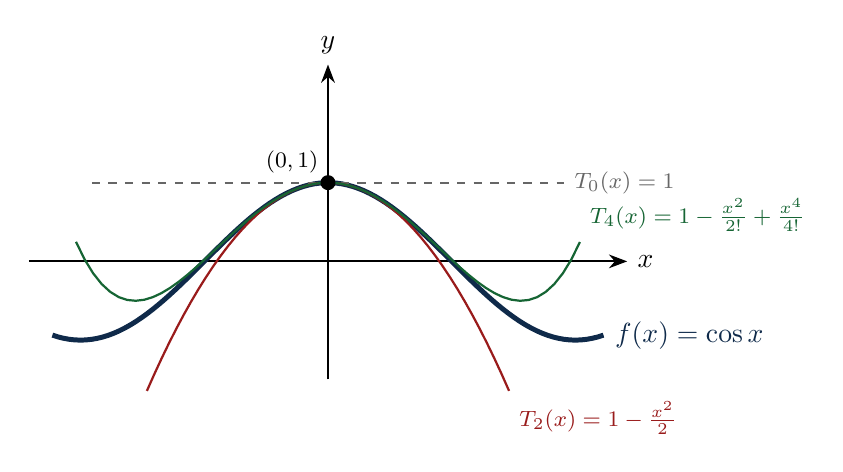
\begin{tikzpicture}[>=Stealth, scale=1.0]
  \definecolor{navyblue}{HTML}{0F2A4A}
  \definecolor{accentcrimson}{HTML}{991B1B}
  \definecolor{forestgreen}{HTML}{166534}
  \definecolor{ambergold}{HTML}{B45309}

  % Axes
  \draw[thick, ->] (-3.8,0) -- (3.8,0) node[right, font=\sffamily\bfseries] {$x$};
  \draw[thick, ->] (0,-1.5) -- (0,2.5) node[above, font=\sffamily\bfseries] {$y$};

  % Exact function: cos(x)
  \draw[line width=1.8pt, navyblue, domain=-3.5:3.5, samples=100] 
    plot (\x, {cos(\x r)}) node[right, font=\sffamily\bfseries] {$f(x) = \cos x$};

  % T0: y = 1
  \draw[thick, dashed, black!60] (-3.0, 1) -- (3.0, 1) node[right, font=\sffamily\footnotesize] {$T_0(x) = 1$};

  % T2: y = 1 - x^2/2
  \draw[thick, accentcrimson, domain=-2.3:2.3, samples=50] 
    plot (\x, {1 - 0.5*\x*\x}) node[below right, font=\sffamily\footnotesize\bfseries] {$T_2(x) = 1 - \frac{x^2}{2}$};

  % T4: y = 1 - x^2/2 + x^4/24
  \draw[thick, forestgreen, domain=-3.2:3.2, samples=60] 
    plot (\x, {1 - 0.5*\x*\x + (1/24)*\x*\x*\x*\x}) node[above right, font=\sffamily\footnotesize\bfseries] {$T_4(x) = 1 - \frac{x^2}{2!} + \frac{x^4}{4!}$};

  \draw[fill=black] (0,1) circle (2.5pt) node[above left, font=\sffamily\footnotesize] {$(0, 1)$};
\end{tikzpicture}
\end{document}